\documentclass{classrep}
\usepackage[utf8]{inputenc}
\frenchspacing

\usepackage{graphicx}
\usepackage[usenames,dvipsnames]{color}
\usepackage[hidelinks]{hyperref}
\usepackage{lmodern}
\usepackage{placeins}
\usepackage{url}
\usepackage{amsmath, amssymb, mathtools}
\usepackage{listings}
\usepackage{fancyhdr, lastpage}

\pagestyle{fancyplain}
\fancyhf{}
\renewcommand{\headrulewidth}{0pt}
\cfoot{\thepage\ / \pageref*{LastPage}}

%--------------------------------------------------------------------------------------%
\studycycle{Informatyka stosowana, studia dzienne, II st.}
\coursesemester{II}

\coursename{Analiza danych złożonych}
\courseyear{2021/2022}

\courseteacher{dr hab inż. Agnieszka Duraj}
\coursegroup{środa, 11:00}

\author{%
    \studentinfo[239671@edu.p.lodz.pl]{Jan Karwowski}{239671}\\
    \studentinfo[239676@edu.p.lodz.pl]{Kamil Kowalewski}{239676}\\
}

\title{Zadanie 1.: Badanie zmienności trendu w strumieniu danych}

\begin{document}
    \maketitle
    \thispagestyle{fancyplain}

    \tableofcontents
    \newpage

    \section{Cel} {
        Celem zadania jest dokonanie analizy charakterystyki strumienia danych pod
        kątem pojawiania sie w nich zmian czyli Detekcja Dryftu.
    }

    \section{Zbiór danych} {
        Zbiorem danych, który został wybrany jest zbiór \emph{Rain in
        Australia}\cite{dataset_weather_aus}. Zawiera on dzienne pomiary pogody z około
        10 lat z różnych stacji badawczych rozmieszczonych w Australii. Zbiór ten
        zawiera jako ostatnią kolumnę klasę \emph{RainTomorrow} z wartościa typu
        Boolean czyli czy będzie jutro padać czy nie. Klasyfikator na podstawie innych
        kolumn dokonuje klasyfikacji a klasa służy do porównania wyniku.

        Zbiór ten wymagał wstępne przygotowania a dokładnie mówiąc dokładna data
        została przekształcona na sam miesiąc pomiaru gdyż uznaliśmy że de facto
        powtarzalne miesiące mogą się przydać podczas klasyfikacji pogody. Co więcej ze
        względu na to, że była 6 kolumn zawierające wartości inne niż liczbowe
        dokonaliśmy ich konwersji przy pomocy \emph{LabelEncoder} z biblioteki
        \emph{sklearn}. Po dokonaniu tych operacji została uruchomiona imputacja i w
        tym przypadku zdecydowaliśmy się na imputację wartością średnią.
    }

    \section{Implementacja} {
        Program został napisany w języku Python z wykorzystaniem biblioteki
        scikit-multiflow\cite{scikit_multiflow} aby skorzystać z gotowych implementacji
        algorytmów do detekcji dryftu i klasyfikacji. Algorytmami, które zostały wybrane
        do detecji dryftu są:
        \begin{itemize}
            \item ADWIN
            \item DDM
            \item KSWIN
            \item PageHinkley
        \end{itemize}
        Jako algorytm klasyfikacyjny został wybrany \textit{KNN} czyli algorytm K
        najbliższych sąsiadów. Do kodu źródłowego jest dołączony skrypt \textit{run.sh}
        zawierający wszystkie kombinacja parametrów użyte do badań natomiast wyniki w
        postaci wykresów są zapisywane do plików.
    }

    \section{Opis algorytmów} {

        \subsection{ADWIN} {
            Algorytm ADWIN\cite{adwin} posiada jeden wymagany parametr a mianowicie
            $\delta \epsilon (0, 1)$, którego zadaniem jest określenie czułości
            algorytmu na detekcje dryftu. Jego działanie polega na dynamicznym
            dostosowaniu rozmiaru okna czasowego poprzez dodawanie kolejnych próbek ze
            strumienia danych. Aby wykryć dryft algorytm porównuje dwa odpowiednio duże
            okna i w przypadku dużych rozbieżności między oknami dryft jest wykrywany.
            Warunkiem zakończenia rozszerzania danego okna jest wykrycie dryft, gdy to
            nastąpi z okna usuwane są stare wartości.
        }

        \subsection{DDM} {
            Algorytm DDM\cite{ddm} opiera się na założeniu, że liczba błedów maleje lub
            pozostaje na tym samym poziomie wraz z ze wzrostem liczby analizowych próbek
            pod warunkiem stacjonarnego rozkładu danych. Celem wyznaczenia progów
            ostrzegawczych i alarmowych, których wzory dla i-tych elementów zostały
            przestawione poniżej,\\

            Próg ostrzegawczy:
            $$
            p_i+s_i \geqslant p_{min}+\textbf{2}*s_{min}
            $$

            Próg alarmowy:
            $$
            p_i+s_i \geqslant p_{min}+\textbf{3}*s_{min}
            $$

            wylicza się stopę błedu, która zawiera wartości $p_{min}$ oraz
            $s_{min}$. Jeśli któryś z warunków przestawiony na powyższych zbiorach
            jest prawdziwy to został przekroczony dany prób. W przypadku przekroczenia
            progu alarmowego można wnioskować, że wystąpił dryft.
        }

        \subsection{KSWIN} {
            Algorytm KSWIN\cite{kswin} jest metodą detekcji dryftu, która opiera się na
            teście statystycznym \emph{Kolmogorov-Smirnov}, który zakłada brak
            zasadniczego rozkładu danych natomiast może monitorować rozkład danych lub
            wydajność. Algorytm ten utrzymuje okno o stałym rozmiarze \emph{n}.
            Ostatnie \emph{r} próbek jest przyjmuję się jako \emph{\textbf{R}}
            natomiast resztę próbek z danego okna czyli o indeksach $n-r$ są jednolicie
            rysowane i są przyjmowane jako \emph{\textbf{W}}. Test ten wykonywany na
            tej samej wielkości oknach \emph{\textbf{R}} oraz \emph{\textbf{W}} i
            porównywany jest dystans rozkładu skumulowanego danych empirycznych
            $dist(R,W)$. Poniżej został przedstawiony po spełnieniu którego zostaje
            wykryty dryft przez algorytm KSWIN.

            $$
            dist(R,W) > \sqrt{-\frac{ln\alpha} {r}}
            $$
        }

        \subsection{PageHinkley} {
            Algorytm PageHinkley\cite{page_hinkley} działa na podstawie obliczania
            średniej z danych przekazanych z wybranego strumienia danych oraz wykorzystuje
            on test statystyczny Page-Hinkley\cite{page_hinkley_test}. Jest tworzona
            hipoteza o braku zmian i jest ona badana poprzez dwa testy celem określenia
            czy wystąpił wzrost czy spadek. Sam test ma określony dopuszczalny próg
            nagłej zmiany średniej wartości. Gdy test wykaże wzrost bądź spadek
            zaprzecza to założonej hipotezie i swiadczy o wystąpieniu znacznej zmiany w
            strumieniu danych.
        }

    }

    \section{Eksperymenty} {

        \subsection{ADWIN} {
            Algorytm ten został zastosowany dwukrotnie, raz z parametrem $\delta=0.01$ a drugi raz z
            $\delta=0.001$. Parametr ten oznacza ,,poziom pewności'', że doszło do zmiany rozkładu
            badanego strumienia - bezpośrednio determinuje czułość działania danej metody. W obu
            przypadkach dla pierwszych 5 tys. próbek ze zbioru danych \emph{nie udało} się wykryć
            dryftu.
        }

        \subsection{DDM} {
            Podobnie jak w przypadku algorytmu ADWIN przeprowadzone zostały dwa eksperymety z
            wykorzystaniem metody DDM. Za każdym razem wykorzystano pierwzse 5 tys. próbek ze zbioru
            danych. Pierwszy eksperyment wykorzystywał domyślne parametry tego algorytmu, drugi
            natomiast zmienił współczynniki we wzorach na ostrzeżenie i detekcję odpowiednio z $2$ i
            $3$ na $1.5$ oraz $2.0$. W ten sposób podczas drugiego eksperymentu czułość działania
            algorytmu została zwiększona. Obrazy \ref{fig:ddm} i \ref{fig:ddm_too_sensitive}
            prezentują dokładność klasyfikacji dla kolejnych próbek, dodatkowo zaznaczone są obszary
            ostrzeżenia o wystąpieniu dryftu oraz sam moment wykrycia. Widać (na rys.
            \ref{fig:ddm_too_sensitive}, że po zmianie wspomnianych parametrów udało się wykryć
            dryft.

            \begin{figure}[!htbp]
                \centering
                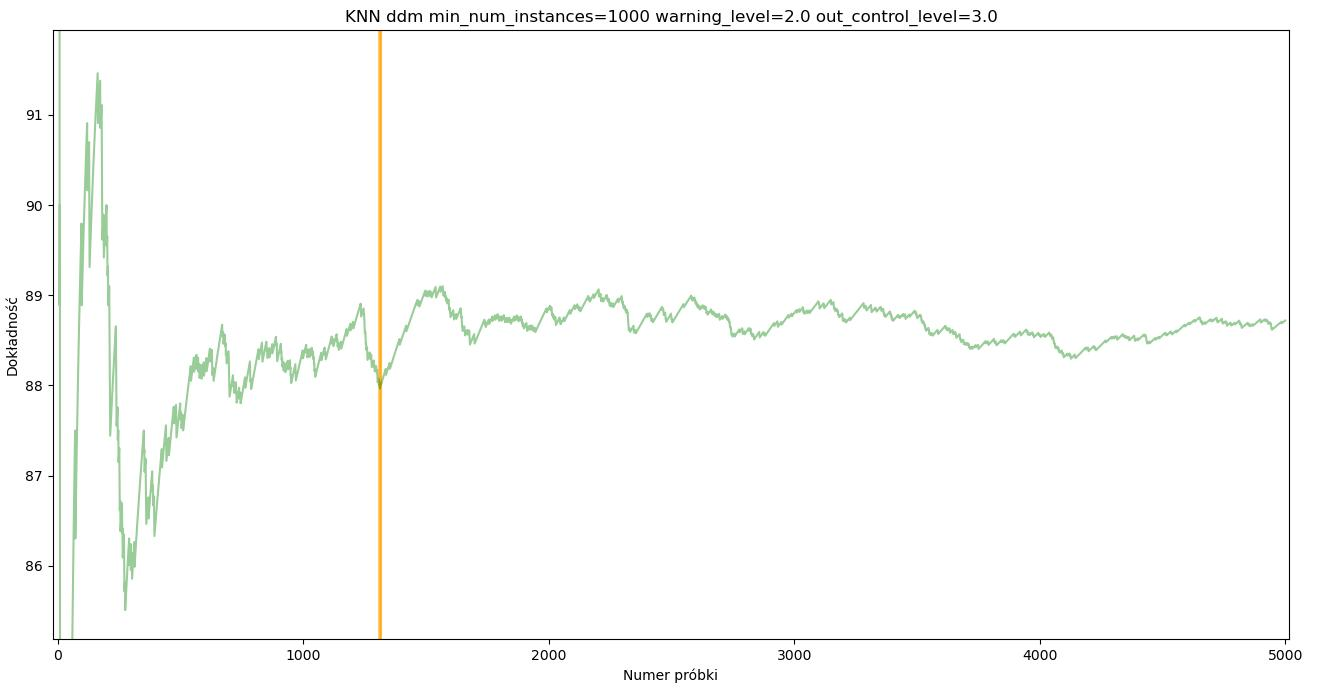
\includegraphics[width=\textwidth]{img/ddm.jpg}
                \caption
                {Wykres dokładności od numeru próbki dla algorytmu DDM, liczba próbek: 5000}
                \label{fig:ddm}
            \end{figure}
            \begin{figure}[!htbp]
                \centering
                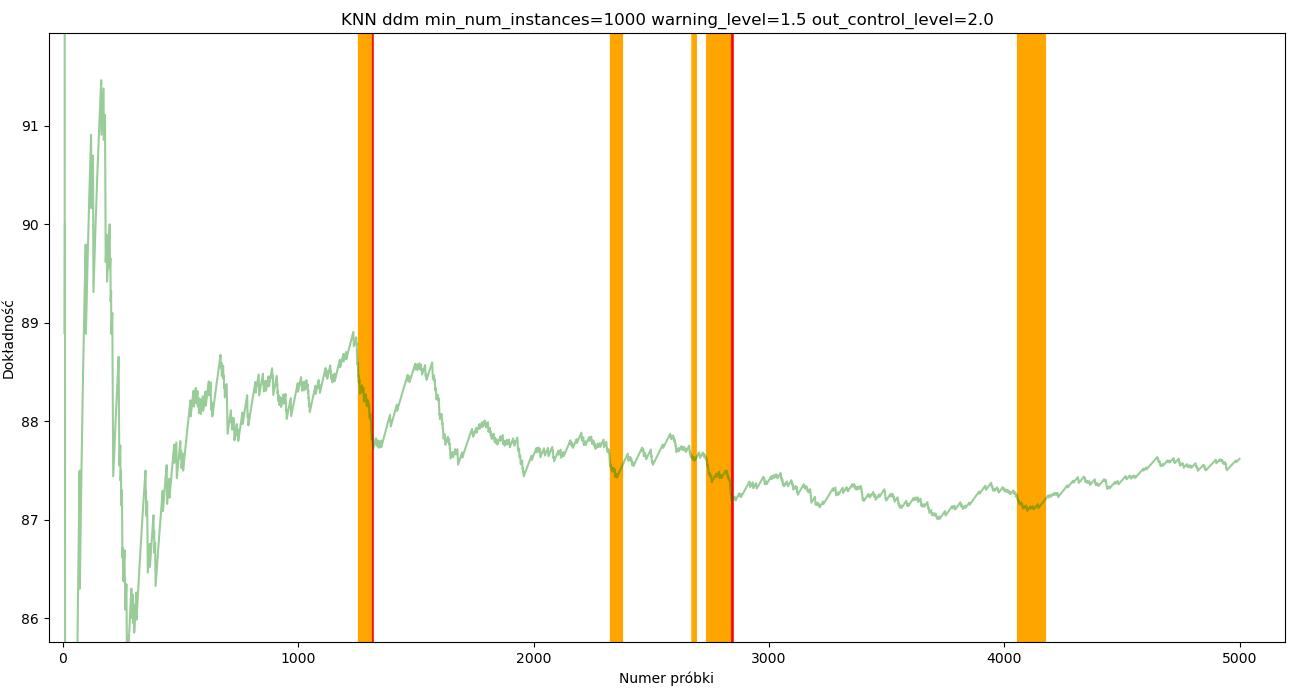
\includegraphics[width=\textwidth]{img/ddm_too_sensitive.jpg}
                \caption
                {Wykres dokładności od numeru próbki dla algorytmu DDM, liczba próbek: 5000}
                \label{fig:ddm_too_sensitive}
            \end{figure}
            \FloatBarrier
        }

        \subsection{KSWIN} {
            W przypadku tego algorytmu nie udało się wykryć dryftu w pierwszych 5 tys. próbek ze
            zbioru danych. Rozmiar okna został ustawiony na $1000$ przykładów a fragment okna
            rozumiany jako najnowsze przykłady składa się z ostatnich $300$ elementów. Parametr
            $\alpha$, determinujący czułość testu statystycznego wykonywanego w ramach tego
            algorytmu, został ustawiony kolejno na wartości 0.001, 0.005 i 0.01. Za żadnym razem nie
            udało się wykryć dryftu.
        }

        \subsection{PageHinkley} {
            Ostatni wykorzystany algorytm to stosunkowo prosta metoda PageHinkley. Ponownie badano
            jedynie pierwszych 5 tys. przykładów ze zbioru danych. Wartości progu detekcji zmian dla
            algorytmu w kolejnych eksperymentach to odpowiednio $50$ i $10$. Był to jedyny zmieniany
            parametr. Za pierwszym razem, kiedy algorytm jest mniej czuły, nie udało się wykryć
            dryftu, po zmianie wartości progu w dwóch miejscach dryft ten stał się zauważalny, co
            prezentuje rys. \ref{fig:ph_too_sensitive}.

            \begin{figure}[!htbp]
                \centering
                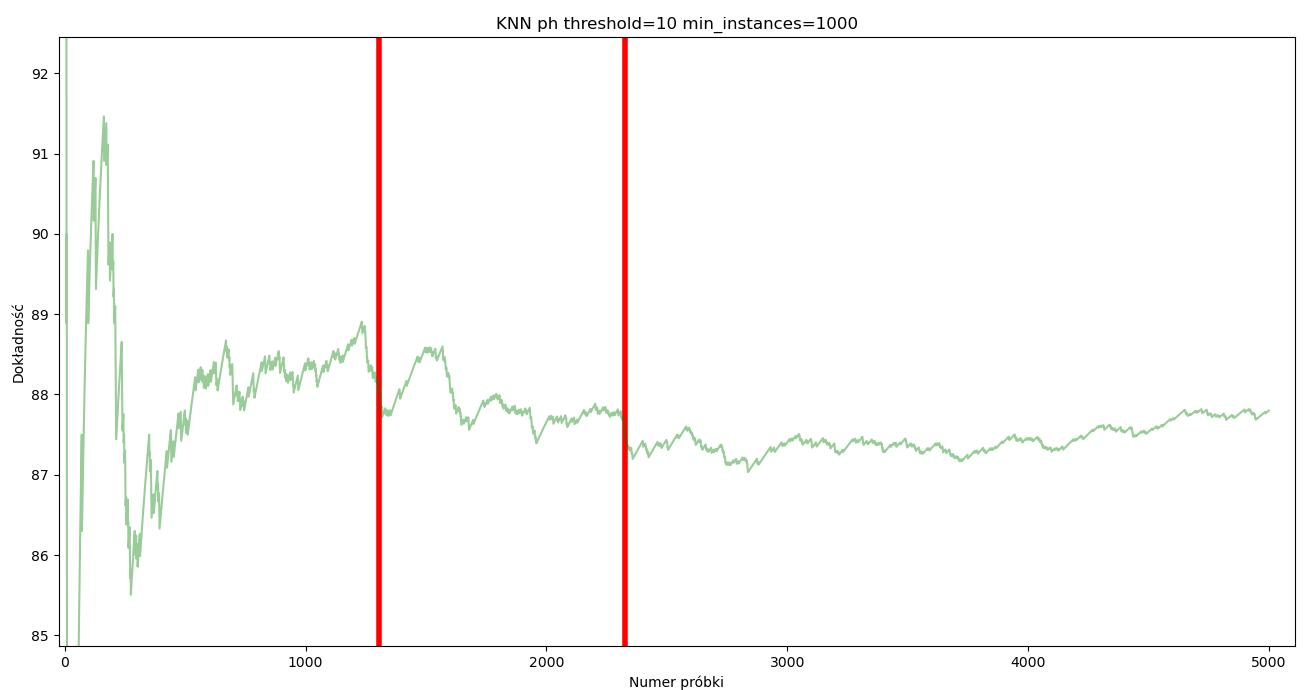
\includegraphics[width=\textwidth]{img/ph_too_sensitive.jpg}
                \caption
                {Wykres dokładności od numeru próbki dla algorytmu PageHinkley, liczba próbek: 5000}
                \label{fig:ph_too_sensitive}
            \end{figure}
            \FloatBarrier
        }
    }

    \section{Dyskusja i wnioski} {
        Przeprowadzone eksperymenty w większości nie wykazały obecności dryftu w wykorzystanym
        zbiorze danych. Co prawda, wykorzystano jedynie niewielkę część całego zbioru i być może
        przy dłuższych badaniach udałoby się taki dryft zlokalizować. Jest jednak prawdopodobne, że
        w tym zbiorze nie jest on obecny, lub jest tak mały, że niezauważalny.

        W przypadku trzech eksperymentów, których wyniki zaprezentowano na wykresach, udało się
        zlokalizować dryft w badanym strumieniu. Nie należy traktować tego jednak jako poprawnego i
        znaczącego wyniku, ponieważ parametry tych algorytmów zostały dobrane tak, aby stały się one
        ,,nadwrażliwe'' na zmiany w rozkładzie dokładności klasyfikacji. Należy zwrócić uwage, że
        dotyczy to dwóch prostszych metod, skupiających się na prostych statystykach obliczonych z
        badanego strumienia. Obie metody oparte o okno (KSWIN oraz ADWIN), mimo manipulacji
        parametrami nie wykazały obecności dryftu w zbiorze danych, co może wskazywać na ich większą
        złożoność, uniwersalność i mniejszą podatność na błędy.

        Ostatecznie wyniki pracy przedstawione w tym sprawozdaniu można podsumować w prostych
        punktach:
        \begin{itemize}
            \item Badany zbiór danych najprawdopodobniej nie posiada zauważalnego dryftu
            \item Pośród badanych metod w dwóch opartych na prostych statystykach łatwo znacząco
                zwiększyć ich czułość i tym samym doprowadzić do niekoniecznie poprawnych wyników
            \item Metody oparte o okno przesówne mimo większej złożoności są zdecydowanie bardziej
                uniwersalne i odporne na błędy, trudniej zwiększyć ich czułość i tym samym łatwiej
                dobrać odpowiednie parametry
        \end{itemize}
    }

    \begin{thebibliography}{0}
        % @formatter:off
        \bibitem{dataset_weather_aus}
        {Kaggle. Rain in Australia. [online]. [dostęp: 28.10.2021]. Dostępny w internecie, URL:
        https://www.kaggle.com/jsphyg/weather-dataset-rattle-package}
        \bibitem{scikit_multiflow}
        {scikit-multiflow. scikit-multiflow. [online]. [dostęp: 23.10.2021].
        Dostępny w internecie, URL: https://scikit-multiflow.readthedocs.io/en/stable/index.html}
        \bibitem{adwin}
        {https://scikit-multiflow.readthedocs.io/en/stable/api/generated/skmultiflow.drift\_detection.\\
        ADWIN.html#skmultiflow.drift\_detection.ADWIN}
        \bibitem{ddm}
        {https://scikit-multiflow.readthedocs.io/en/stable/api/generated/skmultiflow.drift\_detection.\\
        DDM.html#skmultiflow.drift\_detection.DDM}
%        \bibitem{hddm_a}
%        {https://scikit-multiflow.readthedocs.io/en/stable/api/generated/skmultiflow.drift\_detection.\\
%        HDDM\_A.html#skmultiflow.drift\_detection.HDDM\_A}
        \bibitem{kswin}
        {https://scikit-multiflow.readthedocs.io/en/stable/api/generated/skmultiflow.drift\_detection.\\
        KSWIN.html#skmultiflow.drift\_detection.KSWIN}
        \bibitem{page_hinkley}
        {https://scikit-multiflow.readthedocs.io/en/stable/api/generated/skmultiflow.drift\_detection.\\
        PageHinkley.html#skmultiflow.drift\_detection.PageHinkley}
        \bibitem{page_hinkley_test}
        {E. S. Page. 1954. Continuous Inspection Schemes. Biometrika 41, 1/2 (1954), 100–115.}
        % @formatter:on
    \end{thebibliography}

\end{document}
